\documentclass[11pt,a4paper]{article}
\usepackage[T1]{fontenc}
\usepackage[utf8]{inputenc}
\usepackage{lmodern}
\usepackage[margin=2.4cm]{geometry}
\usepackage{microtype}
\usepackage{graphicx}
\usepackage{amsmath,amssymb}
\usepackage{booktabs,tabularx,array}
\usepackage[backend=biber,style=numeric-comp,natbib=true,sorting=none]{biblatex}
\addbibresource{references.bib}
\usepackage{caption}
\usepackage{hyperref}
\hypersetup{colorlinks=true,linkcolor=black,citecolor=black,urlcolor=blue,pdftitle={Frequency-dependent strategic deception in a multiplayer game}}
\newcommand{\CI}[2]{[#1,#2]}
\newcommand{\thetaC}{\theta}
\setlength{\parskip}{0.3em}
\setlength{\parindent}{1.25em}
\captionsetup{font=small,labelfont=bf}
\title{Frequency-dependent strategic deception in a multiplayer hidden-information game with third-party protection}
\author{Antonio Pereira\\\small Federal University of Par\'a, Bel\'em, Brazil\\\small\textit{Authorship and affiliation to be confirmed before submission}}
\date{Manuscript draft, 20 October 2026}
\begin{document}
\maketitle

\begin{abstract}
Deception can benefit a player when opponents accept false claims, but its advantage may change when deception becomes common. We examined this problem in a computational model of \emph{Inten\c{c}\~oes Ocultas}, a multiplayer hidden-information card game in which action claims can be challenged and bystanders may earn a reward for blocking attacks. We compared honest-action agents with agents that consider strategic bluffs, varying scepticism, the frequency of bluffers, the number of players and three models of anticipated protection. In four-player games at low scepticism, a rare bluffer gained 4.4--6.9 percentage points in winning probability relative to an honest resident across belief models. The predicted payoff advantage remained positive at intermediate population frequencies and declined as bluffers became prevalent. Its persistence near an all-bluffer population was uncertain. Three-player results supported a rare-bluffer advantage, whereas five-player results were inconclusive. At high scepticism, agents selected no false actions, making the two strategies behaviourally identical. Increasing the number of bluffers also reduced attacks and successful third-party interventions. These results establish conditional, frequency-dependent selection within a specified computational game. They do not demonstrate human deception or uniquely determine evolutionary stability.
\end{abstract}
\noindent\textbf{Keywords:} evolutionary game theory; strategic deception; bluffing; hidden information; third-party protection; scepticism; agent-based simulation

\section{Introduction}
A false claim can alter another player's decision without changing the underlying distribution of resources or capabilities. Its usefulness depends on the receiver's willingness to challenge, the consequences of a failed claim and the actions available to others. Deception thus has a strategic component: a claim that succeeds in a trusting population can become less profitable when agents expect deception and respond accordingly \citep{searcy2005,mcnally2013}.

The evolutionary analysis of deception has typically used signalling or sender--receiver games in which senders and receivers occupy distinct roles. Capraro and colleagues, for example, demonstrated that the long-run prevalence of lying depends on the payoff structure and the type of lie \citep{capraro2019}. Multiplayer interaction introduces additional decisions. An individual can challenge a claim, defend itself or protect someone else. Those acts are affected by information about other players and by the ordering of the available responses. The link between the private gain from misrepresentation and population-level success is then less direct.

Third-party responses add a second collective problem. Research on indirect reciprocity and norm enforcement has examined the effects of punishment, reputation and helping \citep{fehr2004,leimar2001,raihani2015,rockenbach2006}. If only one bystander may intervene, protection also resembles a volunteer's dilemma \citep{diekmann1985}. In a game with challengeable claims, defenders may bluff about their ability to protect a target, and a challenged false block can still prevent later players from intervening. An attacker must forecast both the possession of a protective card and the decision to claim protection. These expectations can suppress attacks even when actual interventions remain uncommon.

We study these mechanisms using a fully specified simulation of \emph{Inten\c{c}\~oes Ocultas}, a three- to five-player card game with five hidden roles. Each agent chooses resource actions, attacks, challenges and defensive claims from limited public information. Previous development of the model revealed that treating card availability as equivalent to successful blocking produces substantial deterrence without comparable realized protection. Subsequent models used public offer and challenge histories, together with a frozen action-specific calibration. One held-out calibration condition remained outside the prespecified tolerance. The present study retains that model uncertainty as a sensitivity factor.

We ask whether a strategically deceptive policy has a winning advantage when rare, how the advantage changes as deceptive strategies become common and whether the result generalizes across player counts and protective beliefs. Our first analysis compares one potential bluffer with an otherwise identical honest-action control using matched game seeds. We then simulate every mixture of honest and bluffing agents and construct empirical multiplayer payoff tables. Replicator dynamics and finite-population fixation models provide conditional evolutionary projections \citep{taylor1978,gokhale2014,traulsen2007}. The simulations themselves contain no learning across games or reproduction. This separation permits a direct comparison of observed game outcomes and the population-dynamic assumptions used to interpret them.

\section{Methods}
\subsection{Game environment and information structure}
The model follows the Portuguese rulebook for \emph{Inten\c{c}\~oes Ocultas}. Three to five players begin with two hidden influence cards and two coins; the common deck contains three copies each of Regente, Comerciante, Embaixador, Guardi\~ao and Sombra. Revealing both active cards removes a player from the contest. Agents can collect income or external aid, claim a Regente action to collect three coins, claim Comerciante to steal up to two coins, exchange cards as Embaixador, pay three coins to attack as Sombra, or pay seven coins for an unblockable direct coup. A player starting a turn with at least ten coins must execute a coup.

Claims of character-dependent actions can be challenged. The first willing challenger in turn order resolves the claim; the loser of the challenge loses an influence. A targeted Comerciante or Sombra action may be blocked by the target. If the target declines, another active player may intervene in a fixed clockwise order. The first blocking claim, even if exposed as false, precludes subsequent intervention attempts. A successful third-party block earns one coin from the common treasury in the reference condition. Blocks themselves may be challenged. This sequential structure distinguishes the game from a binary sender--receiver interaction and creates an explicit opportunity to measure anticipated and realized protection.

The rule specification used in this study was explicitly approved on 20 October 2026. The last player with at least one active influence wins. Players without active influences become Observers: they may comment informally but cannot act, issue formal challenges, block or intervene. Three coins are paid when a Sombra attack is declared and are not refunded if the attack is challenged, blocked or otherwise unsuccessful. The separate refund experiment is an explicitly counterfactual sensitivity analysis, not an unresolved official rule. For computational termination, the simulator imposes a 400-turn limit and records unfinished games as draws; this cutoff is not a rule of the physical game. Further details appear in the supplementary methods.

\subsection{Agent policies and blocking beliefs}
Two strategy types were compared. Honest-action agents had strategic action-bluff propensity $b=0$. Bluffers had $b=0.8$. This parameter is the probability of \emph{considering} a false character claim; the agent makes that claim only if its estimated value exceeds the best available honest action. Actual false-action frequency can consequently be much smaller than $0.8$ actions per turn. Both strategies retain the same card-counting challenge policy, targeting rule, intervention propensity and defensive policy. The baseline settings were a challenge threshold $\theta\in\{0.05,0.30,0.50\}$, a target-related challenge bonus of $0.15$, intervention propensity $0.5$ conditional on holding a valid protection card, zero voluntary intervention bluffing, and one coin paid for a standing intervention. A last-influence Sombra defense may still be bluffed under an unchanged engine rule. Thus ``honest'' refers to \emph{action claims}, not to every possible defensive utterance.

A challenge is attempted when the observer's probability that the claimant holds the asserted card falls below $\theta$, after the applicable stake bonus. The three public blocking-forecast policies were (i) an empirical rate informed by public past blocking opportunities; (ii) an opponent-aware model pooling public observations with individual-defender histories; and (iii) a frozen action-specific extension that models false-block challenge survival and applies fitted corrections by action and table size. None receives hidden cards or opponents' true policy parameters. The third forecast previously satisfied 11 of 12 held-out action-specific calibration criteria. Its remaining failure concerned three-player Sombra defense; no new coefficients were fitted for the present experiments. Forecast identity is a factor in the design, not a claim that any model is uniquely correct.

We used an experimental counterfactual adapter to prevent a random-stream artifact. The unmodified agent consumes random numbers while considering a rejected bluff, potentially changing later choices even when it never lies. The adapter recomputes the honest action from the same random-generator state and retains the honest generator state whenever a false action is not selected. It changes the agent's random-number bookkeeping, not the valuation of a selected bluff. For rare-mutant pairs in which no false claim occurred, the full recorded game trajectories were identical. Ordinary-agent simulations are retained in the archive as an audit, but the strict-coupling design is the primary contrast.

\subsection{Experiments and statistical design}
The rare-mutant experiment compared one bluffer plus $n-1$ honest residents with $n$ honest agents under matched random seeds, rotating the first-player position relative to the focal player. Each four-player combination of three challenge thresholds and three forecasts used 2,500 matched seed pairs. Each three- and five-player combination used 1,500 pairs. The paired endpoint was the difference in the focal player's probability of winning; 95\% confidence intervals were computed by resampling whole seed pairs. The nine primary four-player hypothesis tests used exact discordant-pair tests with Holm adjustment. The earlier ordinary-agent runs were kept exclusively for the random-stream audit.

The new frequency experiment covered every table composition, $k=0,\ldots,n$ bluffers, with 1,200 independent games per composition. We crossed all three thresholds and three forecasts in four-player games (45 profiles), examined three- and five-player games at $\theta=0.05$ (30 profiles), and varied intervention rewards $r\in\{0,2\}$ at $n=4$, $\theta=0.05$, using the opponent-aware forecast (10 profiles). This gave \textbf{102,000 additional complete-game simulations}. Within a condition, the deck seed was shared across compositions. Strategy subsets and first-player positions were counterbalanced independently: every allocation of $k$ bluffers appeared under every starting position over a repeating block of turns. An earlier pilot with an accidentally phase-locked starting-player schedule was discarded in full before the final analysis.

For each game, we logged the winning strategy, declared false actions, steals and Sombra attacks, intervention offers, claims and standing interventions. The primary frequency endpoint is \emph{per-player} win probability by strategy and table composition. We used 1,500 seed-clustered bootstrap replicates for the displayed frequency-study confidence intervals, resampling the same game-seed index across composition profiles within each condition. The figures additionally display 500-replicate bootstrap bands. The frequency curves, model sensitivity and reward sweep are descriptive and exploratory; we did not assign familywise significance to all 85 profiles.

\subsection{From game outcomes to evolutionary payoffs}
Let $W_B(k)$ denote the number of wins by any bluffer in $G$ games with $k$ bluffers among $n$ players. Define $W_H(k)$ analogously. The empirical payoffs of a \emph{single} player of each type are
\begin{equation}
 u_B(k)=\frac{W_B(k)}{Gk},\qquad u_H(k)=\frac{W_H(k)}{G(n-k)},
 \label{eq:payoffs}
\end{equation}
where each quantity is defined only when the indicated type is present. The invasion advantage of a rare bluffer is $u_B(1)-u_H(0)$; the corresponding advantage near an all-bluffer population is $u_B(n)-u_H(n-1)$. A positive value at the latter boundary indicates resistance to the invasion of rare honest agents. These quantities compare players drawn from the specified population strategy, and do not equate the total wins of $k$ bluffers with the payoff of one bluffer.

Under independent random matching of $n-1$ opponents at population bluffer frequency $x$, the two expected payoffs are
\begin{equation}
\begin{aligned}
 f_B(x)&=\sum_{j=0}^{n-1}\binom{n-1}{j}x^j(1-x)^{n-1-j}u_B(j+1),\\
 f_H(x)&=\sum_{j=0}^{n-1}\binom{n-1}{j}x^j(1-x)^{n-1-j}u_H(j).
\end{aligned}
\label{eq:fitness}
\end{equation}
We report $\Delta(x)=f_B(x)-f_H(x)$ and evaluate the conventional two-type replicator equation $\dot x=x(1-x)\Delta(x)$. Interior roots of $\Delta(x)=0$ are candidate equilibria. Their stability is assessed from the sign of the local derivative, with sampling uncertainty retained. These are \emph{payoff-derived projections}; no population copying or mutation occurs during the card games themselves.

As a second projection, we used the existing finite-population pairwise-comparison model, with population size $M=30$ and Fermi comparison intensity $\beta=5$. It computes fixation probabilities from the same empirical $n$-player payoffs, averaging opponent composition by hypergeometric sampling and treating win probability as a fitness proxy \citep{traulsen2007,omidshafiei2019}. We varied $\beta$ over $0.5$--$10$ to expose its sensitivity. The resulting two-state stationary ranking is a property of this stipulated imitation process and is not a measured rate of evolutionary change in people.

\subsection{Ordered defence as a mechanistic reduction}
The defender order permits a useful decomposition of anticipated protection. For defender $i$ reached in sequence, let $c_i$ be the conditional probability of \emph{claiming} a block and $s_i$ the conditional probability of claiming a block that \emph{stands}. The overall protection probability can be represented as
\begin{equation}
 P(\mathrm{block})=\sum_{i=1}^{m}s_i\prod_{\ell<i}(1-c_\ell),
 \label{eq:ordered}
\end{equation}
provided the conditional probabilities are defined consistently along the sequential offer path. A false block exposed by a challenger contributes to $c_i$ but not $s_i$ and still removes the opportunity for later players. Substituting card ownership for $c_i$ or $s_i$ incorrectly assumes that all eligible card holders will volunteer and that all block claims succeed. Equation~\eqref{eq:ordered} motivates the public offer-history diagnostics without requiring hidden strategy labels.

\section{Results}
\subsection{Rare bluffers benefit from low scepticism}
At $\theta=0.05$, the strict-coupling rare-mutant experiment found increased focal winning probability for a bluffer in four-player games under all three blocking forecasts. The differences were 5.04 percentage points (95\% CI 3.36--6.72) for the empirical forecast, 6.92 (5.24--8.56) for the opponent-aware forecast and 6.28 (4.64--8.00) for the action-specific forecast. All three primary Holm-adjusted tests were significant. The focal bluffer made roughly 2.4--2.5 false action claims per game in these conditions. At $\theta=0.30$, false actions were rare (about 0.02--0.03 per game) and estimated win-rate differences were small. At $\theta=0.50$, no false action was selected, and paired counterfactual trajectories were identical by construction. The evidence concerns a model policy that refuses low-valued bluffs; it is not evidence that challenges defeat every possible deceptive strategy.

\subsection{Frequency-dependent multiplayer payoffs}
The independent composition experiment reproduced a positive rare-bluffer payoff at low scepticism. Table~\ref{tab:primary} reports the selection difference inferred from the profile payoffs, with confidence intervals resampled across game seeds. At a bluffer population frequency of one half, all three models retained a positive advantage. Near the all-bluffer boundary the advantage approached zero or became negative. All three boundary confidence intervals included zero, so the simulations do not establish whether honest players can reliably invade an all-bluffer population.

\begin{table}[htbp]
\centering\small
\caption{Four-player payoff-derived selection difference at low scepticism ($\theta=0.05$), in percentage points of per-player win probability. Intervals are 95\% seed-clustered bootstrap percentile intervals. $\Delta(0)$ is the rare-bluffer advantage; $\Delta(1)<0$ implies a rare honest agent has an advantage in an all-bluffer population.}
\label{tab:primary}
\begin{tabular}{lrrr}
\toprule
Blocking forecast & $\Delta(0)$ & $\Delta(0.5)$ & $\Delta(1)$ \\
\midrule
Empirical & $+4.38$ [1.8, 7.0] & $+3.35$ [1.9, 4.8] & $-0.08$ [-2.5, 2.4] \\
Opponent-aware & $+6.94$ [4.3, 9.6] & $+4.62$ [3.1, 6.1] & $-1.17$ [-3.8, 1.3] \\
Action-specific & $+5.75$ [3.2, 8.2] & $+2.55$ [1.1, 4.0] & $-2.17$ [-4.8, 0.3] \\
\bottomrule
\end{tabular}
\end{table}

\begin{figure}[htbp]
\centering
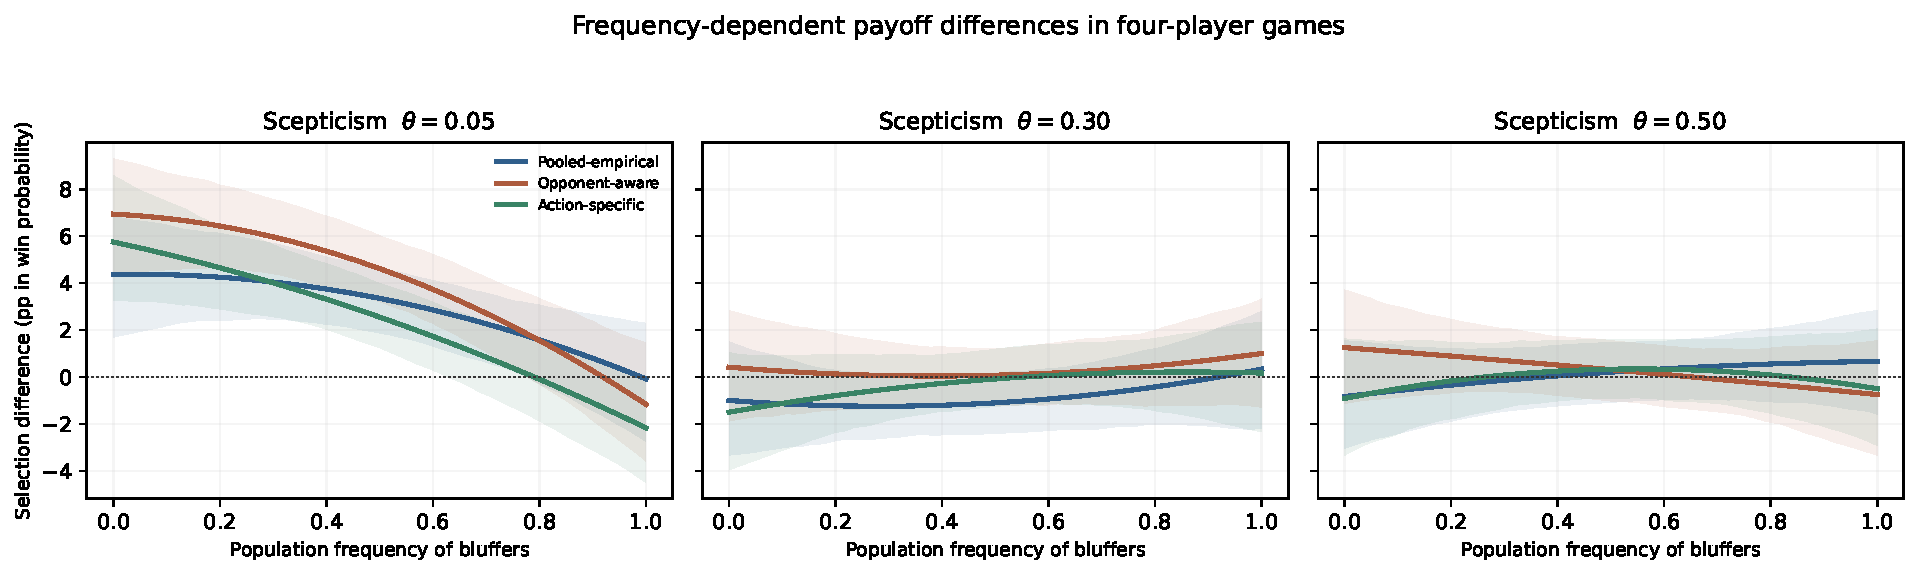
\includegraphics[width=\textwidth]{figures/figure1_selection_by_scepticism.pdf}
\caption{Population-frequency dependence of the payoff difference $f_B(x)-f_H(x)$ in four-player games. Lines are estimates from 1,200 complete games for each of the five possible table compositions, per scepticism level and forecast model. Shading shows 95\% bootstrap uncertainty in the empirical profile payoffs. Positive values favour bluffers under the stipulated random-matching replicator projection. At high scepticism, action policies are behaviourally identical; the small apparent selection differences arise from finite simulation sampling.}
\label{fig:selection}
\end{figure}

The low-scepticism point-estimate curves had interior zeros near $x=0.99$ (empirical), $x=0.92$ (opponent-aware) and $x=0.79$ (action-specific; Figure~\ref{fig:selection}). Their derivative indicated local stability in the plug-in payoff models. However, the bootstrap frequencies of a positive rare-bluffer and negative all-bluffer boundary difference were approximately 51\%, 81\% and 96\%, respectively. Only the action-specific estimate approached a robust interior-root interpretation; none met a strict requirement that both boundary differences exclude zero at 95\% confidence. We consequently treat these roots as \emph{candidate}, not established, evolutionary equilibria.

\begin{figure}[htbp]
\centering
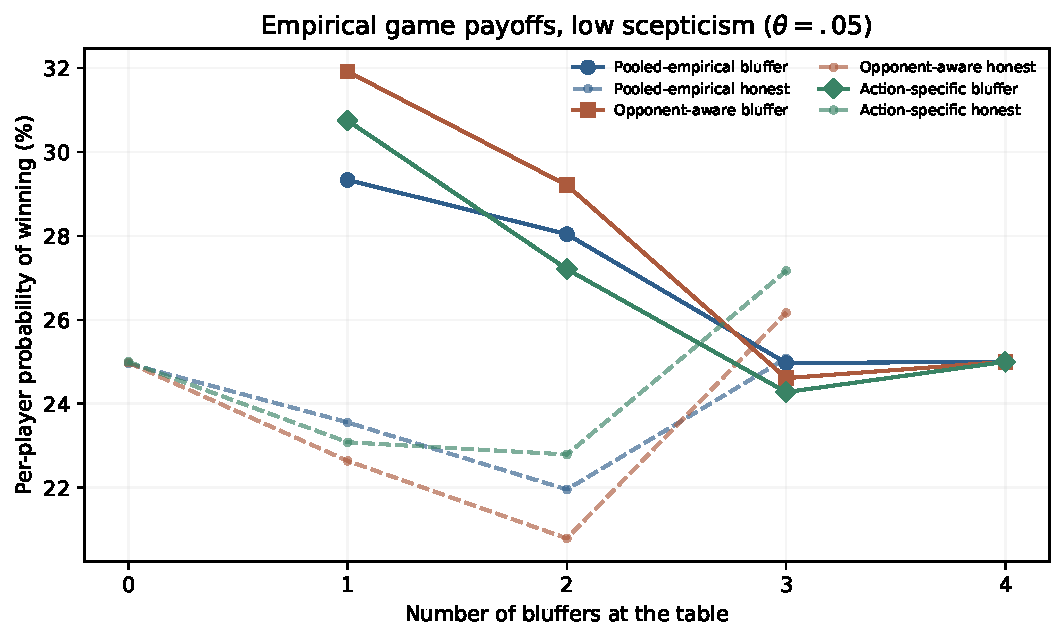
\includegraphics[width=.87\textwidth]{figures/figure2_composition_payoffs.pdf}
\caption{Per-player win probabilities in each of the five four-player strategy compositions at $\theta=0.05$. Solid lines represent bluffers and dashed lines represent honest-action agents. Missing end points indicate that a strategy is absent from the corresponding table. Each estimate is based on 1,200 games with balanced strategy seats and first-player positions.}
\label{fig:payoffs}
\end{figure}

\subsection{Scepticism and table size change the payoff structure}
At $\theta=0.30$, the four-player plug-in rare-bluffer differences ranged from $-1.5$ to $+0.4$ percentage points across forecasts. At $\theta=0.50$, the two policies made exactly the same decisions, with identical winners at every matched seed across all table compositions. The nonzero point-estimate selection curves in that condition are an informative finite-sample negative control, not a behavioural advantage. Inference based only on a point-estimate equilibrium would misinterpret this noise as selection.

At low scepticism, three-player tables showed rare-bluffer advantages of 7.7--9.5 percentage points (all three 95\% intervals above zero). Five-player tables yielded estimates between $-1.6$ and $+0.9$ points (all intervals including zero). In three-player games, the predicted advantage also remained positive near an all-bluffer population. The five-player end-point advantage, by contrast, was positive even where the rare-bluffer estimate was ambiguous. These contrasting profiles suggest that a strategy's capacity to enter a trusting population and its resistance to replacement when prevalent can respond differently to the number of participants. The cross-size comparisons remain exploratory.

\subsection{Deception frequency is associated with fewer attacks and protection events}
Bluffer prevalence changed the mix of actions occurring during play, not merely the winning strategy. Under the opponent-aware model at low scepticism, the average number of false action claims increased from zero in all-honest games to 7.87 in all-bluffer games. Steals and Sombra attacks fell from 2.01 to 0.79 per game; third-party defence offers fell from 1.17 to 0.21, and successfully standing interventions fell from 0.173 to 0.023 (Figure~\ref{fig:protection}). The other two forecasts also showed a decline in attacks as bluffers became more common. These outcomes are generated by endogenous action choice and cannot be interpreted as a direct psychological response to deception by humans.

\begin{figure}[htbp]
\centering
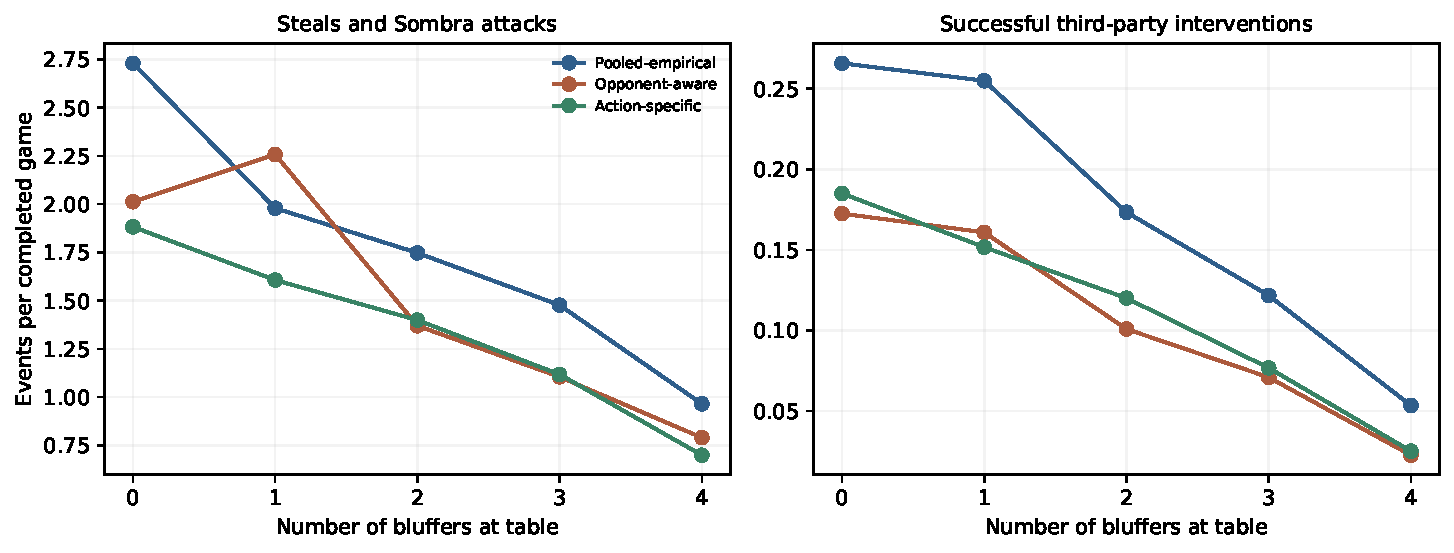
\includegraphics[width=.95\textwidth]{figures/figure3_attack_and_protection.pdf}
\caption{Recorded attack actions (left) and successful third-party interventions (right) per completed four-player game as the number of bluffers increases, at low scepticism and the reference one-coin intervention reward. The decline in protection events largely reflects changing exposure to attacks; it is not evidence that defenders become less willing to help when offered an opportunity.}
\label{fig:protection}
\end{figure}

The additional reward sweep at $r=0,1,2$ retained a positive low-scepticism rare-bluffer advantage under the opponent-aware forecast: $+7.63$, $+6.94$ and $+6.50$ points, respectively. Their 95\% intervals overlapped considerably. This experiment did not isolate the immediate incentive response of a defender, because the simulated intervention propensity is fixed by its strategy parameter. Reward changes may influence future game states without modifying the propensity to intervene at the time of an offer.

The finite-population pairwise-comparison projection ranked bluffers above honest players under low scepticism for all three four-player forecasts, but the magnitude depended strongly on the assumed comparison intensity. With $M=30$, the stationary bluffer probabilities ranged from $0.585$--$0.647$ at $\beta=0.5$ to $0.969$--$0.998$ at $\beta=5$. Those probabilities summarize the postulated imitation process. They are not measured fixation frequencies from evolving populations.

\subsection{Sensitivity to an alternative Sombra cost rule}
Under the alternative rule that refunds a failed Sombra action's three-coin cost, the four-player opponent-aware rare-bluffer advantage at $\theta=0.05$ was $+8.23$ points, compared with $+6.94$ points under the default nonrefund rule. The alternative remained favourable to a rare bluffer. Because the two rule conditions were simulated with different seeds, this numerical difference does not establish that refunds strengthen deception. The confirmed Observer and victory rules were held fixed in all experiments.

\section{Discussion}
The primary finding is a conditional advantage of strategic deception in a population of mostly honest players. That result persists across three alternative models of anticipated protection and appears in independent four-player simulations. As bluffing becomes common, the payoff advantage diminishes. Confidence intervals near the all-bluffer boundary prevent a firm assertion that a stable mixed population exists. The study consequently supports frequency-dependent payoffs while separating the directly observed advantage of a rare strategy from stronger claims about evolutionary stability.

The analysis differs from established sender--receiver models of lying in two respects. First, the decision to misrepresent is embedded in a sequence of competing material actions, so a strategically deceptive agent can decline a lie that offers no improvement over an honest move. Second, attack outcomes depend on target protection and the potential intervention of third parties. Previous studies of deception and cooperation show that the social structure and the distribution of benefits can change which lies are favoured \citep{capraro2019,mcnally2013}. Our results add a finite, ordered multiplayer decision environment in which information and strategic anticipation shape the opportunities for aggression.

The decline in attack frequency warrants particular caution. An observed intervention is the end of a sequence that requires an attack, survival of the action challenge, an available defender and a standing protective claim. If anticipation reduces the first event, realized protection may become rare even with unchanged defender policies. A reward attached to intervention cannot be judged from successful blocks alone. Rates conditional on actually receiving an offer, together with the number of offers, are needed to distinguish willingness from exposure. The ordered-claim representation in equation~\eqref{eq:ordered} also makes clear why the presence of a suitable card is not the same as a successful block.

Table size altered the qualitative payoff profile. Three-player conditions supported an advantage across much of the tested strategy range, while five-player rare invasion was inconclusive. This may reflect changing target opportunities, resource accumulation, card distributions or strategic competition. The present design cannot isolate a single mediator. Particularly in five-player games, a successful false claim need not translate into final victory. Future experiments should condition success on claim type and game state, or manipulate attack opportunity independently of the population composition.

The conclusions have several explicit boundaries. Agent action scores rely on fixed coin-equivalent influence values and a restricted target-choice heuristic. Their challenge rules are deterministic thresholds based on public card counts, not a validated model of human belief revision. One action-specific blocking calibration stratum previously failed an independent holdout criterion, and some forecast variants generate different endogenous attack distributions. At $\theta=0.50$, the fitted decision rule selects no false actions, creating a genuine behavioural equivalence of the two parameter types; an unconditional or compelled-deception policy could produce a different result. The reported frequency payoffs are drawn from finite match samples. Replicator equilibria and Fermi fixation probabilities apply only after an additional assumption about matching and the conversion of winning probability into reproductive or imitative success. Selection intensity, the set of candidate strategies and the population structure were not learned from data.

The approved reference rules now specify observer participation, victory and the nonrefundable Sombra cost. We tested only a counterfactual refund after a failed action challenge; alternative observer or victory mechanisms were outside the study's scope. Conclusions therefore apply to the specified rules and should not be assumed to hold in games adopting different conventions. Finally, no human participants were studied. Strategic deception in a deterministic artificial policy cannot establish psychological motives or behaviour in real social settings.

The model nonetheless supplies a tractable research design. It separates a player's option to lie from the willingness of others to believe and the opportunities of third parties to intervene. The current findings motivate a next empirical test in which human subjects face controlled levels of scepticism and manipulated protection opportunities, with challenge decisions and offers recorded separately. Such a protocol would test the behavioural premises that remain stipulated here.

\section{Conclusion}
Strategic bluffing increased winning probability when rare in trusting three- and four-player simulated populations. Its advantage weakened as bluffers became common, and the five-player rare-invasion results did not establish a comparable gain. The effect of anticipation on aggression and protection could be observed directly, while claims of evolutionary stability remained conditional on uncertain payoff estimates and specified update dynamics. The essential computational result is the dependence of deception's payoff on population composition, scepticism and information about defence.

\section*{Data accessibility and code}
The frozen simulator, experimental scripts and summary payoff tables are stored in the private \texttt{squareshorts/intencoes-ocultas} review branch. Seed-level simulation outputs accompany the present reproducibility archive. \textbf{Before journal submission}, code, data and the versioned manuscript should be placed in a publicly accessible repository with a persistent identifier; a public archive DOI has not been assigned. The existing historical Experiments~2--4 remain unchanged and are not presented as confirmatory evidence for this article.

\section*{Ethics}
This work uses computer simulations only and includes no human or animal participants. There was no collection of personal information.
\section*{Funding, competing interests and contributions}
Author contributions, funding and competing-interest declarations require confirmation before submission. Computational and editorial assistance from generative AI should be disclosed according to the target journal's policies.

\printbibliography
\end{document}
